\section{Document conventions}

\begin{figure}[ht]
  \centering
  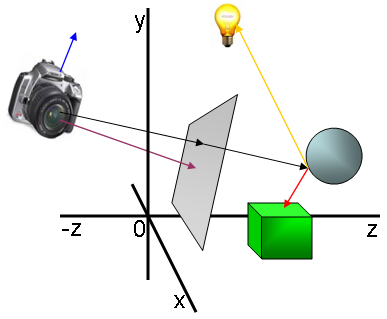
\includegraphics[height=7cm]{img/intro.png}
  \caption{Ray tracing}
\end{figure}

\begin{itemize}
  \item eye : camera
  \item viewport : plan where the eye is looking at
  \item shading effect : way to render/color a pixel (ray intersection with an object)
  \item scene : the scene the ray tracer have to render (described in the xml scene file)
\end{itemize}

